\documentclass[12pt]{article}
\usepackage[utf8]{inputenc}
\usepackage[T1]{fontenc}
\usepackage[polish]{babel}
\usepackage{amsmath} 
\usepackage{amssymb} 
\usepackage{array} 
\usepackage{amsthm,amsfonts}
\usepackage{graphicx}
\usepackage[utf8]{inputenc}
\usepackage[T2A]{fontenc} 


\title{Systemy Liczbowe}
\author{Andrij Andrijczuk}
\date{\today}

\begin{document}

\newtheorem*{thm}{Twierdzenie}
\newtheorem*{rmk}{Uwaga}
\newtheorem*{ex}{Przykład}
\newtheorem*{defi}{Definicja}
\newtheorem*{alg}{Algorytm}

\maketitle

\section{Wprowadzenie do systemów liczbowych} 

\large
{
Systemy liczbowe to zbiory zasad i symboli używanych do zapisywania i przedstawiania liczb. Zanim stały się dla nas tak powszechne, przeszły wiele zmian i przekształceń. Każdy region miał swój własny system liczbowy, który z czasem ewoluował i się udoskonalał. O tych najczęściej spotykanych i najpowszechniej używanych opowiem dzisiaj.
}

\bigskip

\section{Pierwsze systemy liczbowe}

\subsection{Najstarszy znany system liczbowy}
\large
{
Nie jest możliwe jednoznaczne wskazanie, który system liczbowy był pierwszy, ale jednym z najstarszych, który wciąż jest z nami, jest liczenie na palcach. To ono doprowadziło do pojawienia się systemu dziesiętnego (o podstawie 10) oraz piątkowego (o podstawie 5) w wielu kulturach.
}

\newpage

\subsection{Liczenie za pomocą nacięć}
\large
{
Kiedy brakło palców, dla większej wygody, nasi przodkowie zaczęli robić nacięcia na kijach lub kościach. Jednymi z najstarszych znalezisk, które o tym świadczą, są Kość Lebombo i Kość Ishango.
}

\bigskip

\begin{figure}[h]
    \caption{Kość Lebombo i kość Iszango}
    \centering
    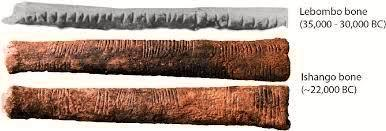
\includegraphics[width=13cm]{Lebombo Bone image.jpeg}
    \label{fig:Lebombo Bone image.jpeg}
\end{figure}

 
\begin{rmk}
{Każde nacięcie oznacza jedną jednostkę liczenia.}
\end{rmk}

\newpage

\section{Systemy dodawania liczb}
\large
{
Później pojawiały się bardziej zaawansowane systemy liczbowe: starożytny egipski (około 3100 r. p.n.e.) i rzymski (około 1000 r. p.n.e.)
}


\begin{center}
\begin{table}[h]
    \caption{Starożytny egipski system liczbowy}
\begin{tabular}{| c | c | c | c |} 
    \hline 
    Liczba & Starożytny hieroglif egipski & Liczba & Starożytny hieroglif egipski \\ 
    \hline 
    1 & $
\includegraphics[width=0.4cm]{Line_1.png}$ & 10000 & $
\includegraphics[width=0.25cm]{Finger_10000.png}$ \\ 
    \hline 
    10 & $
\includegraphics[width=0.4cm]{Loop_10.png}$ & 100000 & $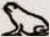
\includegraphics[width=0.8cm]{Frog_100000.png}$ \\ 
    \hline 
    100 & $
\includegraphics[width=0.6cm]{Spiral_100.png}$ & 1000000 & $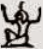
\includegraphics[width=0.8cm]{God_1000000.png}$ \\ 
    \hline 
    1000 & $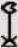
\includegraphics[width=0.4cm]{Lotos_1000.png}$ & & \\ 
    \hline 
\end{tabular}
\end{table}[h]
\end{center}

\begin{center}
\begin{table}[h]
    \caption{Starożytny rymski system liczbowy}
\begin{tabular}{| c | c | c | c |} 
    \hline 
    Liczba & Starożytny hieroglif rzymski & Liczba & Starożytny hieroglif rzymski \\ 
    \hline 
    1 & I & 100 & C \\ 
    \hline 
    5 & V & 500 & D \\ 
    \hline 
    10 & X & 1000 & M \\ 
    \hline 
    50 & L &  &  \\ 
    \hline 
\end{tabular}
\end{table}[h]
\end{center}

\newpage

\begin{quote}
    Mnożenie dwóch liczb w systemie rzymskim sprawia znacznie większe trudności, a niekiedy było wręcz niemożliwe, nawet dla Rzymian! Jeśli chcemy obliczyć 3444 $\cdot$ 394 musimy odwołać się do zapisów wprowadzonych w średniowieczu.[1]
\end{quote}

\textbf{Mnożenie}

\begin{tabular}{rcll}
\multicolumn{2}{l}{\strut 3444} & $\rightarrow$ & MMMCDXLIV \\
$\cdot$ & \strut 394 & $\rightarrow$ & CCCXCIV \\
\multicolumn{2}{r}{\strut = 1 356 936} & $\rightarrow$ & \overline{M}CCC\overline{L}VXCMXXXVI \\
\end{tabular}


\section{Pozycyjne systemy liczbe}
\large
Wymyślenie pozycyjnego systemu liczbowego było w tamtych czasach prawdziwą rewolucją. Wartość symbolu w końcu zależała od jego pozycji, co pozwoliło na efektywne zapisywanie ogromnych liczb i umożliwiło skomplikowane obliczenia.

Jest to zasługa ludów sumeryjskich i babilońskich. To właśnie ich osiągnięcie możemy zobaczyć dzisiaj, po prostu sprawdzając, która jest godzina, ponieważ te narody przyczyniły się do wynalezienia sześćdziesiętnego systemu liczbowego, którym ludzkość do dziś mierzy czas.

Wspominając pozycyjny system liczbowy, nie można pominąć narodów arabskich i indyjskich, które udoskonaliły ten system, dodając do niego nic, czyli zero.

\newpage

\section{Binarne system }
\large

Ostatni, ale nie mniej ważny, jest dwójkowy system liczbowy.
Jest to jeden z najmłodszych systemów liczbowych, który ludzkość wynalazła stosunkowo niedawno, aby roboty i komputery również mogły prowadzić logiczne obliczenia i przekazywać wyniki nam, swoim użytkownikom. Sam system składa się tylko z dwóch symboli – cyfr 0 i 1, które powtarzają się, tworząc tekst zrozumiały dla komputera.

\begin{ex}
\begin{equation*}
0\,1\,0\,0\,1\,0\,0\,0\,\,\,\,\,0\,1\,1\,0\,1\,0\,0\,1\,\,\,\,\,0\,0\,1\,0\,0\,0\,0\,1\,\,-\,Hi!
\end{equation*}
\end{ex}

\newpage

\section{Podsumowanie}
\large

W tej prezentacji opowiedziałem nie o wszystkich istniejących systemach liczbowych, ale starałem się omówić najważniejsze momenty, na których opierała się cała ludzkość. Dziękuję za uwagę!


\begin{thebibliography}{9}

\bibitem{Crilly2009} % <-- Мітка, яку можна використовувати для посилань \cite{...}
Crilly, T. (2009). \textit{50 teorii matematyki, które każdy powinien znać}. PWN, Warszawa.

% Тут можуть бути інші джерела
% \bibitem{Smith2020} Smith, J. (2020). Tytuł książki. Wydawnictwo, Miasto.

\end{thebibliography}


\end{document}
